%% ---------------------------------------------------------------------------
%%  BDhighresDA -- arXiv preprint
%%  Zero-shot generative data assimilation for 5 km daily precipitation
%%  over Bangladesh.
%%
%%  Build:  pdflatex BDhighresDA_arxiv.tex  (x2)
%%
%%  TODO before posting:
%%    - fill in affiliation/ORCID on line ~60
%%    - fill in the code + data availability URLs in Sec. "Availability"
%%    - record wall-clock training and sampling cost (Table 6, last row)
%% ---------------------------------------------------------------------------
\documentclass[10pt,twocolumn]{article}

\usepackage[T1]{fontenc}
\usepackage{lmodern}          % scalable fonts: required for microtype expansion
\usepackage[letterpaper,margin=0.72in,columnsep=0.25in]{geometry}
\usepackage{amsmath,amssymb}
\usepackage{booktabs,multirow,array}
\usepackage{graphicx}
\usepackage[dvipsnames]{xcolor}
\usepackage{microtype}
\usepackage{enumitem}
\usepackage{caption}
\usepackage{url}
\usepackage{hyperref}
\usepackage{tikz}
\usetikzlibrary{arrows.meta,positioning,fit,backgrounds,calc,shapes.geometric}

\hypersetup{
  colorlinks=true,
  linkcolor=MidnightBlue,
  citecolor=MidnightBlue,
  urlcolor=MidnightBlue,
  pdftitle={Zero-shot generative data assimilation for 5 km daily precipitation over Bangladesh: observing-system experiments and a controlled real-data protocol},
  pdfauthor={Fahad Abdullah}
}

\setlength{\parindent}{1em}
\setlength{\parskip}{0pt}
\setlist{nosep,leftmargin=*}
\captionsetup{font=small,labelfont=bf}
\newcommand{\dd}{\,\mathrm{d}}
\newcommand{\mmday}{\mathrm{mm\,day^{-1}}}
\newcolumntype{L}[1]{>{\raggedright\arraybackslash}p{#1}}
\newcolumntype{R}[1]{>{\raggedleft\arraybackslash}p{#1}}
\newcommand{\us}{\_\allowbreak}
\newcommand{\scr}[1]{\texttt{\footnotesize #1}}

%% --- figure palette (shared by Fig. 1) -------------------------------------
\definecolor{cData}{HTML}{2F5C8F}
\definecolor{cProc}{HTML}{0F7A6B}
\definecolor{cModel}{HTML}{B0512E}
\definecolor{cObs}{HTML}{6A4C9C}
\definecolor{cEval}{HTML}{A33A5B}

\title{\bfseries Zero-Shot Generative Data Assimilation for 5\,km Daily
Precipitation over Bangladesh:\\[2pt]
\large Observing-System Experiments and a Controlled Real-Data Protocol}

\author{Fahad Abdullah\\
\small George Mason University, Fairfax, Virginia, USA\\
\small \texttt{fahadabdullaah@gmail.com}}
\date{\today}

\begin{document}

\twocolumn[{%
\maketitle
\begin{center}\begin{minipage}{0.93\textwidth}
\small\noindent\textbf{Abstract.}
\noindent
Bangladesh has no continuous 5\,km daily rainfall analysis: the available
information is split between a coarse gauge analysis, an atmospheric
reanalysis, satellite footprints, and roughly one rain gauge per
4{,}200\,km$^2$. We build and stress-test a probabilistic
0.05$^\circ$ framework that keeps statistical downscaling and observation
assimilation strictly separate. A conditional rectified-flow U-Net learns
$p(x\mid c)$, a distribution over fine-scale precipitation corrections to a
0.5$^\circ$ CPC field, conditioned on five ERA5 state variables, terrain,
position and season. The network never sees a gauge or a satellite pixel.
At inference it is frozen, and Bangladesh Meteorological Department (BMD)
gauges and 0.1$^\circ$ IMERG footprints enter only through differentiable
likelihood guidance, so the observing network and its error model can change
without retraining.
In an observing-system simulation experiment, near-perfect pseudo-observations
cut withheld-station CRPS from 6.94 to 1.12~$\mmday$ and raise
sub-footprint correlation from 0.010 to 0.444, establishing that fine-scale
information really is recoverable through the operators. Realistic
pseudo-observation errors cut the same score only to 4.77~$\mmday$ and leave
the ensemble under-dispersive. We then run a controlled May 2018 real-data
experiment with exact 03:00--03:00\,UTC accumulation windows and five disjoint
spatial station folds. Gauge-only assimilation attains the best pooled CRPS
(4.638~$\mmday$) and gauge\,$+$\,IMERG fusion is close but worse
(4.878~$\mmday$); with five days of data neither the difference nor the
fold-win count is statistically resolvable, so we select gauge-only
provisionally rather than declaring fusion refuted. Because May 2018 lies
inside the prior's training period, we present this as \emph{process}
validation, not product validation. The paper is written to be reproduced and
falsified: it reports the failed ablations alongside the successful ones,
states the alignment bug that changed the conclusion, and specifies the
full-month, bias-corrected and temporally independent tests that must pass
before a Bangladesh rainfall product can be claimed.
\end{minipage}\end{center}
\vspace{1.6em}
}]

\section{Introduction}

Daily rainfall over Bangladesh is set by monsoon flow, Bay of Bengal moisture
transport, organized convection, and sharp orographic gradients near the
Meghalaya Plateau and the Chittagong Hill Tracts. A coarse gridded analysis
represents the synoptic setting but cannot determine where, within a 50\,km
cell, the rain actually fell. A satellite product resolves spatial
organization at about 0.1$^\circ$ but carries retrieval, sampling, timing and
regime-dependent errors. National rain gauges measure directly but are far too
sparse to define a continuous field.

The problem is therefore not interpolation. It is to estimate a
\emph{distribution} over plausible 0.05$^\circ$ precipitation fields,
conditioned on a coarse atmospheric state and on heterogeneous observations
with genuinely different error structures. A useful system must (i) improve
scores at gauges it has never seen, (ii) keep realistic spatial variability
rather than blurring convection, (iii) quantify its own uncertainty honestly,
and (iv) stay modular when stations close or a satellite version changes.

We address this with a conditional generative prior and zero-shot data
assimilation. The prior is a rectified-flow downscaler trained without any BMD
or IMERG input. At inference, observations steer the frozen sampler through
their physical operators and error models. The construction follows the idea
of using a generative model as a non-Gaussian prior for an inverse
problem~\cite{chung2023,rozet2023sda} and, in the geoscientific setting, the
km-scale station assimilation of Manshausen et al.~\cite{manshausen2025},
with the diffusion trajectory replaced by flow
matching~\cite{lipman2023,liu2023,albergo2023}.

\paragraph{Contributions.}
\begin{enumerate}[label=(\arabic{enumi})]
\item A reproducible 0.5$^\circ$\,$\rightarrow$\,0.05$^\circ$ probabilistic
downscaling and posterior-sampling pipeline for Bangladesh, in which the
learned prior and the observation model are separable by construction
(Fig.~\ref{fig:workflow}).
\item Exact temporal and spatial observation operators for BMD gauges and
half-hourly IMERG, including the 48-interval 03:00--03:00\,UTC accumulation
that a BMD reporting day actually denotes.
\item An OSSE that separates two failure modes usually conflated in
generative-DA papers: an ensemble can be simultaneously \emph{too energetic}
at fine scales and \emph{too narrow} in the set of storm placements it samples.
\item A controlled real-data protocol with predeclared, withheld-gauge
selection criteria, and an explicit account of the ablations that failed ---
dense satellite over-constraint, error inflation, sequential fusion, and a
background-date offset that changed the headline result.
\end{enumerate}

\paragraph{What this paper does not claim.}
It does not claim a validated Bangladesh rainfall product. The real-data
evidence is five days inside the prior's training window, and the differences
between the leading methods are smaller than the uncertainty we can currently
attach to them (\S\ref{sec:power}). It does not claim that satellite fusion
fails; it claims that fusion has not yet cleared a gate that a five-day
experiment is capable of adjudicating. It does not claim calibration: both the
OSSE and the real folds fail at least one dispersion diagnostic.

\begin{figure*}[t]
\centering
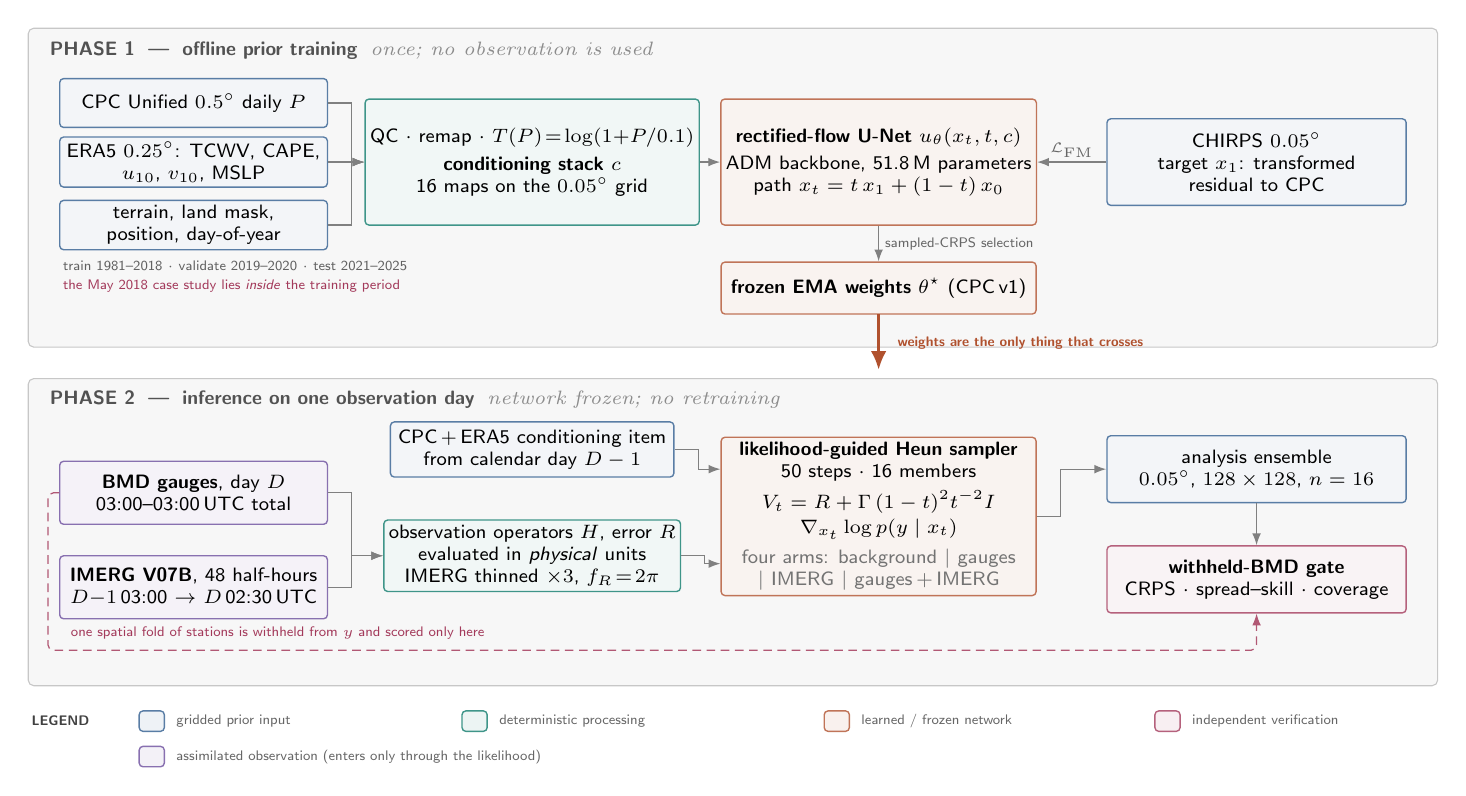
\begin{tikzpicture}[
  x=1mm,y=1mm,
  font=\sffamily\scriptsize,
  box/.style={rounded corners=1.4pt,draw,line width=0.5pt,align=center,inner sep=1.8pt},
  dat/.style ={box,draw=cData!80,fill=cData!6},
  prc/.style ={box,draw=cProc!80,fill=cProc!6},
  mdl/.style ={box,draw=cModel!80,fill=cModel!7},
  obs/.style ={box,draw=cObs!80,fill=cObs!7},
  evl/.style ={box,draw=cEval!80,fill=cEval!6},
  tag/.style ={font=\sffamily\tiny,text=black!60,align=center,inner sep=1pt},
  band/.style={rounded corners=2pt,draw=black!22,fill=black!3,line width=0.4pt},
  bandlab/.style={font=\sffamily\scriptsize\bfseries,text=black!68,anchor=west},
  a/.style   ={-{Latex[length=1.5mm,width=1.1mm]},draw=black!50,line width=0.45pt},
  awt/.style ={-{Latex[length=2.4mm,width=2mm]},draw=cModel,line width=1.2pt},
  aeval/.style={-{Latex[length=1.5mm,width=1.1mm]},draw=cEval!85,line width=0.45pt,
                dash pattern=on 1.1mm off 0.7mm,rounded corners=2pt},
]
\begin{scope}[on background layer]
  \fill[band] (0,55.5) rectangle (179,96);
  \fill[band] (0,12.5) rectangle (179,51.5);
\end{scope}
\node[bandlab] at (1.5,93.2)
  {PHASE 1\; ---\; offline prior training\; \textcolor{black!45}{\normalfont\itshape once; no observation is used}};
\node[bandlab] at (1.5,48.8)
  {PHASE 2\; ---\; inference on one observation day\; \textcolor{black!45}{\normalfont\itshape network frozen; no retraining}};

\node[dat,minimum width=34mm,minimum height=6.2mm] (cpc) at (21,86.5) {CPC Unified $0.5^\circ$ daily $P$};
\node[dat,minimum width=34mm,minimum height=6.2mm] (era) at (21,79) {ERA5 $0.25^\circ$: TCWV, CAPE,\\ $u_{10}$, $v_{10}$, MSLP};
\node[dat,minimum width=34mm,minimum height=6.2mm] (sta) at (21,71) {terrain, land mask,\\ position, day-of-year};

\node[prc,minimum width=36mm,minimum height=16mm] (pack) at (64,79)
  {QC $\cdot$ remap $\cdot$ $T(P)\!=\!\log(1{+}P/0.1)$\\[2pt]
   \textbf{conditioning stack $c$}\\ 16 maps on the $0.05^\circ$ grid};

\node[mdl,minimum width=40mm,minimum height=16mm] (unet) at (108,79)
  {\textbf{rectified-flow U-Net} $u_\theta(x_t,t,c)$\\[2pt]
   ADM backbone, 51.8\,M parameters\\
   path $x_t=t\,x_1+(1-t)\,x_0$};

\node[dat,minimum width=38mm,minimum height=11mm] (chirps) at (156,79)
  {CHIRPS $0.05^\circ$\\ target $x_1$: transformed\\ residual to CPC};

\draw[a] (cpc.east) -- ++(3,0) |- (pack.west);
\draw[a] (era.east) -- (pack.west);
\draw[a] (sta.east) -- ++(3,0) |- (pack.west);
\draw[a] (pack) -- (unet);
\draw[a] (chirps) -- node[tag,above=0.2mm]{$\mathcal{L}_{\mathrm{FM}}$} (unet);

\node[mdl,minimum width=40mm,minimum height=6.6mm] (frozen) at (108,63)
  {\textbf{frozen EMA weights} $\theta^\star$ (CPC\,v1)};
\node[tag,anchor=west,align=left,text=black!62] at (4,64.5)
  {train 1981--2018 $\cdot$ validate 2019--2020 $\cdot$ test 2021--2025\\[1pt]
   \textcolor{cEval}{the May 2018 case study lies \emph{inside} the training period}};
\draw[a] (unet) -- node[tag,right=0.4mm]{sampled-CRPS selection} (frozen);

\draw[awt] (108,59.7) -- (108,52.6);
\node[tag,text=cModel,anchor=west,font=\sffamily\tiny\bfseries] at (110,56)
  {weights are the only thing that crosses};

\node[obs,minimum width=34mm,minimum height=8mm] (bmd) at (21,37)
  {\textbf{BMD gauges}, day $D$\\ 03:00--03:00\,UTC total};
\node[obs,minimum width=34mm,minimum height=8mm] (imerg) at (21,25)
  {\textbf{IMERG V07B}, 48 half-hours\\ $D{-}1$\,03:00 $\rightarrow$ $D$\,02:30\,UTC};

\node[dat,minimum width=36mm,minimum height=7mm] (item) at (64,42.5)
  {CPC\,+\,ERA5 conditioning item\\ from calendar day $D-1$};
\node[prc,minimum width=36mm,minimum height=9mm] (opr) at (64,29)
  {observation operators $H$, error $R$\\ evaluated in \emph{physical} units\\ IMERG thinned $\times3$, $f_R\!=\!2\pi$};

\node[mdl,minimum width=40mm,minimum height=20mm] (samp) at (108,34)
  {\textbf{likelihood-guided Heun sampler}\\ 50 steps $\cdot$ 16 members\\[3pt]
   $V_t=R+\Gamma\,(1-t)^2t^{-2}I$\\[1pt]
   $\nabla_{x_t}\log p(y\mid x_t)$\\[3pt]
   \textcolor{black!55}{four arms: background $|$ gauges}\\
   \textcolor{black!55}{$|$ IMERG $|$ gauges\,$+$\,IMERG}};

\node[dat,minimum width=38mm,minimum height=8.5mm] (ens) at (156,40)
  {analysis ensemble\\ $0.05^\circ$, $128\times128$, $n=16$};
\node[evl,minimum width=38mm,minimum height=8.5mm] (ver) at (156,26)
  {\textbf{withheld-BMD gate}\\ CRPS $\cdot$ spread--skill $\cdot$ coverage};

\draw[a] (bmd.east)   -- ++(3,0) |- (opr.west);
\draw[a] (imerg.east) -- ++(3,0) |- (opr.west);
\draw[a] (item.east)  -- ++(3,0) |- ([yshift=6mm]samp.west);
\draw[a] (opr.east)   -- ++(3,0) |- ([yshift=-6mm]samp.west);
\draw[a] (samp.east)  -- ++(3,0) |- (ens.west);
\draw[a] (ens) -- (ver);
\draw[aeval] (bmd.west) -- (2.5,37) -- (2.5,17) -- (156,17) -- (ver.south);
\node[tag,text=cEval,anchor=west,font=\sffamily\tiny] at (5,19.2)
  {one spatial fold of stations is withheld from $y$ and scored only here};

\node[tag,anchor=west,text=black!75,font=\sffamily\tiny\bfseries] at (0,8){LEGEND};
\foreach \x/\c/\t in {14/cData/{gridded prior input}, 55/cProc/{deterministic processing},
                      101/cModel/{learned / frozen network}, 143/cEval/{independent verification}}
  {\node[box,draw=\c!80,fill=\c!8,minimum width=3.2mm,minimum height=2.6mm,anchor=west] at (\x,8){};
   \node[tag,anchor=west] at (\x+4.4,8){\t};}
\node[box,draw=cObs!80,fill=cObs!8,minimum width=3.2mm,minimum height=2.6mm,anchor=west] at (14,3.5){};
\node[tag,anchor=west] at (18.4,3.5){assimilated observation (enters only through the likelihood)};
\end{tikzpicture}
\caption{End-to-end workflow. The prior learns a stochastic transformed-space
correction from CPC and ERA5 to CHIRPS resolution; no gauge or satellite
observation exists anywhere in Phase 1, so the only quantity crossing into
Phase 2 is the weight vector $\theta^\star$. At inference the network is
frozen: a BMD archive day is paired with exactly 48 half-hourly IMERG
intervals (Eq.~\ref{eq:imergsum}), while the complete CPC--ERA5 conditioning
item is taken from the \emph{preceding} calendar day, because 21 of the 24
observation hours fall there (\S\ref{sec:timing}). Gauge and satellite terms
guide one trajectory through a composite likelihood. Only stations excluded
from that likelihood are allowed to rank methods.}
\label{fig:workflow}
\end{figure*}

\section{Related work}

\paragraph{Generative downscaling of precipitation.}
Deterministic regression to a fine grid produces the conditional mean, which
for rainfall is over-smooth and systematically under-represents the extremes
that matter for flood risk. Generative approaches replace it with a sample
from $p(x\mid c)$. GAN-based super-resolution of atmospheric
fields~\cite{leinonen2021}, generative downscaling of precipitation
forecasts~\cite{harris2022}, deep generative nowcasting from
radar~\cite{ravuri2021}, and diffusion-based km-scale downscaling
(CorrDiff)~\cite{mardani2024} all establish that sampled fields recover
realistic texture and sharper extremes than a conditional mean. All of them,
however, ingest their observations as \emph{predictors}: the network must be
retrained if the observing system changes.

\paragraph{Generative models as priors for inverse problems.}
Diffusion posterior sampling~\cite{chung2023} evaluates a Gaussian likelihood
at the denoised endpoint estimate and differentiates it through the network,
which converts an unconditional generative model into an approximate posterior
sampler for arbitrary differentiable forward operators. Score-based data
assimilation applies this to dynamical
systems~\cite{rozet2023sda,rozet2023}, and Manshausen et
al.~\cite{manshausen2025} apply it to km-scale weather with sparse stations.
Our contribution relative to that line is not the estimator but the
\emph{protocol}: a heterogeneous, real observing system (point gauges plus
dense correlated satellite footprints) with exact accumulation windows, and a
selection rule enforced at withheld stations.

\paragraph{Flow matching.}
Rectified flow~\cite{liu2023} and flow
matching~\cite{lipman2023,albergo2023} learn a velocity field along a linear
probability path, which is cheaper to sample than a diffusion trajectory and
admits exact algebraic conversion between the learned velocity and the score
(Appendix~\ref{app:score}). That identity is what allows a DPS-style
likelihood correction to be applied to a flow model without approximation.

\paragraph{Precipitation verification.}
We use the fair (unbiased) ensemble CRPS estimator~\cite{ferro2014,zamo2018},
CRPS as a proper score~\cite{gneiting2007,hersbach2000}, rank
histograms~\cite{hamill2001}, and the fractions skill
score~\cite{roberts2008}. For paired score differences on serially correlated
daily fields, a block bootstrap~\cite{politis1994} is required; we return to
this in \S\ref{sec:power}.

\section{Data and study design}

\subsection{Domain and grids}

The production Bangladesh grid contains $128\times128$ cell centres at
0.05$^\circ$, spanning 87.6--94.0$^\circ$E and 20.3--26.7$^\circ$N. Training
uses random $128\times128$ crops from a $256\times256$ WIDE grid spanning
84.0--96.8$^\circ$E and 16.0--28.8$^\circ$N. Latitudes are stored ascending.
A training crop is rejected unless at least 30\% of it is land, which removes
nearly all-ocean targets. Grid edges lie on multiples of 0.1$^\circ$, so every
0.05$^\circ$ cell nests exactly inside one IMERG footprint --- this is what
makes the satellite forward operator exact rather than interpolated
(\S\ref{sec:operators}).

\subsection{Gridded predictors and target}

Table~\ref{tab:data} summarizes the streams. CHIRPS supplies the 0.05$^\circ$
daily training target and is gauge-informed~\cite{funk2015}. CPC Unified is a
contemporaneous gauge analysis, not a forecast; its global 0.5$^\circ$ field is
bilinearly mapped to the fine grid and paired with an explicit validity
channel~\cite{chen2008}, with missing precipitation stored as finite zero and
validity zero. ERA5 contributes total-column water vapour, CAPE, 10-m zonal
and meridional wind, and mean sea-level pressure~\cite{hersbach2020}. The
operational CPC-conditioned checkpoint deliberately excludes ERA5
precipitation, because CPC already supplies the coarse precipitation base and
including both invites the network to learn a shortcut between two gauge
analyses. Seven static fields provide square-root-scaled elevation,
standardized slope, the land mask, and four longitude/latitude positional
encodings; sine and cosine of day-of-year add seasonality.

The configured temporal split is 1981--2018 for training, 2019--2020 for
validation, and 2021--2025 for testing. \textbf{The May 2018 experiment
therefore falls inside the training period.} This is a deliberate choice ---
it is the only month for which the legacy BMD archive, the half-hourly IMERG
windows and the trained checkpoint were all simultaneously available --- and
it is the single most important constraint on how the real-data results may be
read (\S\ref{sec:limits}).

\begin{table*}[t]
\centering
\caption{Data streams and their roles. ``Prior'' means a model input available
during training and inference; ``observation'' means the stream enters only the
inference-time likelihood and never the network.}
\label{tab:data}
\small
\begin{tabular}{L{0.14\textwidth}L{0.11\textwidth}L{0.13\textwidth}L{0.14\textwidth}L{0.32\textwidth}}
\toprule
Stream & Native scale & Time support & Role & Processing used here \\
\midrule
CHIRPS v2 & 0.05$^\circ$, daily & 1981 onward & Prior training target; OSSE nature run & Selected onto the exact fine grid; used only as context in real-data verification, because it is gauge-informed and it trained the prior~\cite{funk2015}. \\
CPC Unified & 0.5$^\circ$, daily & 1979 onward & Coarse precipitation prior & Bilinear remapping plus a validity channel; transformed-space residual base~\cite{chen2008}. \\
ERA5 & 0.25$^\circ$, hourly & 1940 onward & Atmospheric prior & Daily means of TCWV, CAPE, $u_{10}$, $v_{10}$, MSLP; all five fields move together in timing tests~\cite{hersbach2020}. \\
IMERG Final V07B & 0.1$^\circ$, half-hourly & Satellite era & Dense observation & 48 rates accumulated to each BMD reporting day; exact $2\times2$ footprint operator; native random error propagated~\cite{huffman2020}. \\
BMD gauges & Point, daily & Historical station archive & Sparse observation and \emph{primary} validation & Legacy station-month matrix converted to a long daily table; spatially disjoint holdout folds. \\
Copernicus GLO-90 & $\sim$90\,m, static & Static & Terrain prior & Area-aggregated to 0.05$^\circ$ before elevation and slope features are derived. \\
\bottomrule
\end{tabular}
\end{table*}

\subsection{BMD observations and the reporting day}

The historical BMD archive is a station-month matrix with day-of-month columns
and explicit missing markers; station identifiers and coordinates come from a
separate catalogue. Invalid calendar cells, negative values, values above
1000~mm and missing markers are removed, and known spelling variants are
reconciled explicitly. May 2018 yields 930 valid station-days from 30
stations, a 54.7\% wet-station-day fraction, and a maximum of 179~$\mmday$.

A BMD archive date $D$ denotes a 24-h accumulation ending at 03:00~UTC
(09:00 Bangladesh Standard Time). The matching satellite observation is
therefore
\begin{equation}
 P_D^{\mathrm{IMERG}} = \sum_{k=1}^{48} r_k\,(0.5~\mathrm{h}),
 \label{eq:imergsum}
\end{equation}
where interval starts run from $D-1$ 03:00 through $D$ 02:30~UTC and $r_k$ is
in mm\,h$^{-1}$. The random-error depth is propagated as the root of the sum
of the 48 squared half-hourly error depths. All 48 unique intervals are
mandatory: an incomplete or duplicated window fails preprocessing rather than
being rescaled, because a silently rescaled window is indistinguishable from a
correct one downstream. May 1--31 requires 1{,}488 files, beginning 30 April at
03:00 and ending 31 May at 02:30. Equation~\eqref{eq:imergsum} already crosses
the UTC date boundary, so IMERG is \emph{not} shifted by an additional day.

For the bounded experiment, a deterministic farthest-point algorithm creates
geographically dispersed holdouts. An initial split assimilates 24 stations and
withholds six. The stronger gate partitions all 30 stations into five disjoint
spatial folds, so every station is withheld exactly once and every method is
scored on identical station-days.

\section{Method}

\subsection{Conditional rectified-flow prior}

Let $x_1$ denote the standardized, transformed fine-grid precipitation
correction and $x_0\sim\mathcal{N}(0,I)$. The linear probability path is
\begin{equation}
 x_t = t x_1 + (1-t)x_0, \qquad t\in(0,1),
 \label{eq:path}
\end{equation}
so that $x_t\mid x_1 \sim \mathcal{N}\!\left(t x_1,(1-t)^2 I\right)$. The
U-Net $u_\theta(x_t,t,c)$ receives the noisy state, continuous time, and the
conditioning stack $c$, and regresses the velocity $x_1-x_0$:
\begin{equation}
 \mathcal{L}_{\mathrm{FM}}=
 \mathbb{E}\!\left[\left\|M\odot\{u_\theta(x_t,t,c)-(x_1-x_0)\}\right\|_2^2\right],
 \label{eq:flowloss}
\end{equation}
where $M$ masks invalid ocean cells and $t$ is drawn from a logit-normal
distribution~\cite{esser2024}, which concentrates training effort at
intermediate noise levels. The target is a residual to CPC rather than an
absolute field,
\begin{equation}
 x_1 = \frac{T(P_{\mathrm{CHIRPS}})-T(P_{\mathrm{CPC}})-\mu_r}{\sigma_r},
 \label{eq:residual}
\end{equation}
so that a zero physical correction reproduces CPC rather than climatology.
Operational v1 uses $T(P)=\log(1+P/0.1)$, with $0.1$~mm approximately the BMD
reporting resolution, followed by training-only standardization.

The clean endpoint estimates are algebraic consequences of
Eq.~\eqref{eq:path}:
\begin{equation}
 \widehat{x}_1=x_t+(1-t)u_\theta,\qquad
 \widehat{x}_0=x_t-t\,u_\theta .
 \label{eq:endpoints}
\end{equation}
Heun integration transports independent noise draws to an ensemble of
fine-grid corrections~\cite{karras2022}. Results reported from the OSSE used
30 sampler steps; the current DA configuration uses 50. We retain and report
per-run sampler metadata rather than silently attributing an old result to the
latest configuration.

\subsection{Architecture and checkpoint provenance}

Every result below comes from a single checkpoint,
\texttt{runs/prior\_h100\_cpc/best.pt}, referred to as CPC~v1. A newer
configuration, CPC~v2, is implemented but has not produced any number in this
paper; Table~\ref{tab:architecture} states the difference explicitly so that
architectural work which has not been rerun cannot be credited with existing
DA scores.

Both versions use an ADM-style U-Net~\cite{dhariwal2021} with a 96-channel
stem and multipliers $[1,2,3,4]$, giving resolution/channel pairs $128/96$,
$64/192$, $32/288$ and $16/384$. Each encoder level has two residual blocks;
the decoder has three after skip concatenation. Residual blocks use
GroupNorm~\cite{wu2018}, SiLU, $3\times3$ convolutions, dropout 0.2 and
Fourier-time FiLM scale/shift~\cite{perez2018}. Self-attention is applied at
32 and 16 pixels and in the middle block, with four heads. Downsampling is a
stride-2 $3\times3$ convolution; upsampling is nearest-neighbour interpolation
followed by a $3\times3$ convolution. The v1 conditioning stack has 16 maps:
seven dynamic, seven static, two seasonal.

CPC~v1 is trained for 150 epochs with AdamW, learning rate
$1.5\times10^{-4}$, weight decay 0.01, 2{,}000 warmup steps then cosine decay,
unit gradient clipping, batch size 32 and EMA decay 0.9995. Conditioning
dropout is zero and classifier-free guidance~\cite{ho2022cfg} is fixed at one,
so the reported checkpoint is a purely conditional downscaler and not a jointly
trained unconditional model. Checkpoint selection uses sampled validation CRPS
where available, never training flow loss alone.

\begin{table*}[t]
\centering
\caption{The checkpoint that produced every reported result, versus the latest
implemented configuration. Keeping these columns apart is what prevents
un-rerun architectural improvements from being credited with existing DA
scores.}
\label{tab:architecture}
\small
\begin{tabular}{p{0.20\textwidth}p{0.35\textwidth}p{0.36\textwidth}}
\toprule
Component & \textbf{CPC v1} --- source of all results here & CPC v2 --- implemented, not yet rerun \\
\midrule
Backbone & 96-channel ADM U-Net; multipliers 1/2/3/4; attention at 32 and 16; four heads; $\approx$51.8\,M parameters & Same core widths and attention; $\approx$57.5\,M parameters \\
Condition injection & All 16 condition maps concatenated at the model input & Input concatenation plus a learned condition pyramid injected at every U-Net scale through zero-initialized $1\times1$ residual projections \\
Precipitation transform & Log1p for the CPC and CHIRPS residual & Square root for the CPC and CHIRPS residual \\
Objective & Masked flow-matching velocity loss & Flow loss plus 0.5$^\circ$ coarse-consistency (weight 0.10) and CPC consistency (weight 0.02) \\
Sampling emphasis & Uniform daily sampling, random valid crops & 35\% top-decile wet-day mixture; 50\% chance of targeting a top-5\% wet pixel in a crop \\
Validation monitor & Sampled CRPS on EMA weights; best checkpoint near epoch 40 & Fifteen fixed July cases stratified over precipitation quantiles \\
\bottomrule
\end{tabular}
\end{table*}

\subsection{Zero-shot likelihood guidance}
\label{sec:guidance}

Let $y$ stack the observations and let $H$ map a candidate fine field to
observation space. The target posterior is
\begin{equation}
 p(x\mid y,c)\;\propto\;p_\theta(x\mid c)\,p(y\mid x).
 \label{eq:posterior}
\end{equation}
Following diffusion posterior sampling~\cite{chung2023}, at trajectory time
$t$ we evaluate a Gaussian likelihood at the endpoint estimate
$H(\widehat{x}_1)$,
\begin{equation}
 \log p(y\mid x_t) = -\tfrac{1}{2}
 \left[y-H(\widehat{x}_1)\right]^{\!\top}\! V_t^{-1}
 \left[y-H(\widehat{x}_1)\right]+\mathrm{const},
 \label{eq:likelihood}
\end{equation}
\begin{equation}
 V_t=R+\Gamma\,\frac{(1-t)^2}{t^2}\,I .
 \label{eq:vt}
\end{equation}
Here $R$ is the observation-error covariance (\S\ref{sec:operators}) and
$\Gamma$ is a single scalar controlling how strongly the endpoint estimate is
distrusted early in the trajectory. The $(1-t)^2/t^2$ factor is not
arbitrary: inverting Eq.~\eqref{eq:path} for $x_1$ given $x_t$ under a flat
prior gives exactly $\operatorname{Var}(x_1\mid x_t)=\frac{(1-t)^2}{t^2}I$, so
Eq.~\eqref{eq:vt} inflates $R$ by a scaled version of the true endpoint
uncertainty. We use $\Gamma=10^{-3}$, consistent with the value
Manshausen et al.~\cite{manshausen2025} found preferable for precipitation.

The likelihood gradient is differentiated through both the U-Net and the
observation operator, clipped for stability, and converted from a score
correction to a velocity correction by the factor $(1-t)/t$. That factor is
exact for a linear interpolant; Appendix~\ref{app:score} derives it. The
practical consequence is that observations exert almost no influence while the
trajectory is mostly noise, and approach their specified error weight near the
clean endpoint.

The experiment has four matched arms: \emph{background} (no likelihood),
\emph{gauges}, \emph{IMERG}, and \emph{simultaneous} (gauges $+$ IMERG). Every
ensemble member receives independently perturbed observations; IMERG
perturbations are spatially correlated. ``Simultaneous'' means the gauge and
satellite likelihood terms are concatenated within one guided trajectory --- it
is not a two-stage analysis. All four arms share random seeds, so differences
between them isolate the effect of the likelihood.

\subsection{Observation operators and error model}
\label{sec:operators}

The gauge operator converts a candidate from transformed model space to
physical precipitation, bilinearly samples the 0.05$^\circ$ grid at each
station, and returns to transformed observation space. The IMERG operator
likewise acts in physical units and takes the exact mean of each nested
$2\times2$ block of fine cells. Averaging in \emph{physical} space is
essential: the precipitation transform is nonlinear, so the transform of a
block mean is not the block mean of the transform, and the error incurred by
confusing the two is largest exactly where rainfall is heaviest.

Gauge $R$ combines measurement variance with point-to-grid representativeness
variance; for a point gauge compared against a 5\,km daily average of
convective rainfall, the representativeness term dominates. IMERG $R$ uses the
propagated native \texttt{randomError}, a transformed-space floor, and a
representativeness term. To avoid treating thousands of spatially correlated
satellite pixels as independent, the experiment retains every third
0.1$^\circ$ footprint in each direction. With correlation length $\ell=3$
coarse cells and stride $s=3$, the diagonal variance is multiplied by
\begin{equation}
 f_R=\max\!\left[1,\,2\pi(\ell/s)^2\right]=2\pi\approx6.28 ,
 \label{eq:rinflate}
\end{equation}
retaining 356 land footprints per day. This is an effective-sample-size
approximation, not a claim that the residual covariance is diagonal; its
inadequacy is one candidate explanation for the fusion result in
\S\ref{sec:folds}. No fitted IMERG bias correction is applied anywhere in this
paper, which is a known and material omission (\S\ref{sec:limits}).

\subsection{Verification protocol and predeclared gates}
\label{sec:gates}

The primary score is fair ensemble CRPS at BMD stations withheld from the
likelihood~\cite{gneiting2007,ferro2014}. Deterministic RMSE, MAE, bias and
correlation use the ensemble mean. We also report spread--skill ratio, 90\%
interval coverage, rank histograms~\cite{hamill2001}, Brier scores and
reliability at 1, 10, 25 and 50~$\mmday$, critical success index, day/station
error matrices, and collocated CPC, raw IMERG, CHIRPS and
inverse-distance-weighted gauge baselines.

Two rules are enforced throughout, and both were fixed before the rotated-fold
run was executed:

\begin{enumerate}[label=\textbf{G\arabic{enumi}.}]
\item \textbf{Only withheld gauges rank methods.} CHIRPS agreement and map
sharpness are descriptive context. CHIRPS is gauge-informed \emph{and} trained
the prior, so a method that matches CHIRPS better may simply be reproducing
its own training signal.
\item \textbf{A method must win on pooled CRPS and on at least three of five
folds} to displace the incumbent.
\end{enumerate}

Gate G2 is weaker than it appears, and we say so in \S\ref{sec:power} rather
than leaving it to the reader.


\section{Experiment 1: observing-system simulation}
\label{sec:osse}

\subsection{Design}

The OSSE treats independent held-out July CHIRPS fields as a 0.05$^\circ$
nature run. Exact $2\times2$ means form pseudo-IMERG footprints; a
farthest-point design places 40 pseudo-stations, of which 20\% are withheld.
Thirty days and 16 ensemble members are used, and background and analysis share
random seeds so that any difference isolates assimilation.

Two observation regimes are run. The \emph{near-perfect} regime retains only a
small numerical error floor and asks whether the operators and guidance can
reconstruct information across scales at all. The \emph{realistic} regime adds
the configured gauge and correlated-satellite errors and is the meaningful
stress test. Both remain optimistic, because a CHIRPS-on-CHIRPS construction
omits real satellite and gauge biases and all product mismatch; the OSSE
bounds what is achievable, it does not predict real skill.

\subsection{Results}

Table~\ref{tab:osse} summarizes the runs. With near-perfect observations,
withheld CRPS falls by 83.9\%, full-field CRPS from 8.276 to 1.836~$\mmday$,
and subgrid RMSE from 5.170 to 4.444~$\mmday$; subgrid correlation rises from
0.010 to 0.444. Since a 0.1$^\circ$ footprint mean contains no information
about the arrangement of rainfall inside it, a subgrid correlation of 0.444
can only have come from the prior --- this is direct evidence that the frozen
generative prior supplies fine-scale structure that the observations do not
carry.

With realistic errors, withheld CRPS still improves by 31.2\%, but full-field
improvement collapses to 9.6\%. The spread--skill ratio is 0.51 and
rank-histogram deviation is 0.392: the ensemble is strongly under-dispersive.
At the same time the member-to-truth fine-scale power ratio reaches 5.98.

These last two numbers are the most useful thing the OSSE produced, because
they are usually reported as if they were the same defect and they are not. A
power ratio near six means an individual member is \emph{too rough} --- it
paints small-scale texture that the truth does not have. A spread--skill ratio
of 0.51 means the \emph{set} of members is too narrow --- the 16 fields
disagree less than they should about where and how hard it rained. A system
can have both at once, and this one does: it manufactures high-wavenumber
noise while remaining overconfident about the placement and amplitude of
storms. Fixes aimed at one make the other worse if applied blindly, which is
why we report them separately rather than as a single ``calibration'' verdict.

\begin{table*}[t]
\centering
\caption{OSSE results, transcribed from remote run reports. CRPS values are in
$\mmday$. A spread--skill ratio below one indicates an ensemble that is too
narrow relative to its realized error.}
\label{tab:osse}
\small
\begin{tabular}{L{0.21\textwidth}L{0.11\textwidth}L{0.12\textwidth}L{0.23\textwidth}L{0.17\textwidth}}
\toprule
Metric & Realistic errors & Near-perfect errors & Interpretation & Verdict \\
\midrule
Withheld CRPS, background $\rightarrow$ analysis & 6.94 $\rightarrow$ 4.77 & 6.94 $\rightarrow$ 1.12 & 31.2\% and 83.9\% improvement & \textbf{Pass} \\
Full-field CRPS improvement & 9.6\% & 77.8\% & Realistic errors sharply reduce the spatial benefit & Pass only near-perfect \\
Innovation standard deviation & 1.03 & 1.10 & Close to the unit-normalized target & Pass \\
Spread/skill ratio & 0.51 & 0.59 & Both ensembles are under-dispersive & \textbf{Fail} \\
Rank-histogram deviation & 0.392 & 0.569 & Substantial non-uniformity & \textbf{Fail} \\
Land cells improved & 70.1\% & 89.5\% & Majority of cells improve & Pass \\
Subgrid RMSE, background $\rightarrow$ analysis & --- & 5.170 $\rightarrow$ 4.444 & Fine-scale residual becomes more accurate & Pass \\
Subgrid correlation, background $\rightarrow$ analysis & --- & 0.010 $\rightarrow$ 0.444 & Information added \emph{below} footprint scale & \textbf{Pass} \\
Analysis 90\% coverage & --- & 0.807 & Improved, still below nominal 0.90 & Marginal \\
Fine-scale power, member/truth & 5.98 & 1.00 (background 1.54) & Realistic members are too energetic at fine scales & \textbf{Fail} realistic \\
\bottomrule
\end{tabular}
\end{table*}

\section{Experiment 2: May 2018 real observations}

The bounded real design uses May 1--5, 2018; exact half-hour IMERG windows;
the $D-1$ complete CPC--ERA5 prior item; 16 members; four arms; and five
disjoint spatial folds, giving 150 withheld station-days across 30 stations.

\subsection{Temporal alignment changed the conclusion}
\label{sec:timing}

The first dense-satellite experiment produced a catastrophic fused CRPS of
15.07~$\mmday$, against 10.79 for the background and 4.74 for gauges alone.
Thinning footprints and inflating $R$ stabilized the likelihood but did not
fix the underlying mismatch. In the superseded calendar-day experiment,
simultaneous CRPS was 6.587 and a sequential IMERG-then-gauge update was
8.142, both far worse than gauges alone at 4.742. Raising total satellite $R$
inflation from 6.3 to 50.3 monotonically improved simultaneous CRPS from 6.587
to 5.203 --- and that is precisely the diagnostic signature of a misaligned
constraint. Weakening a satellite term until it stops hurting is not the same
as extracting information from it; the limit of that process is the gauge-only
solution.

Two corrections changed the picture. First, rebuilding the accumulation from
240 half-hourly files, so that each BMD day is the exact 48-interval window of
Eq.~\eqref{eq:imergsum}, improved IMERG-only CRPS from 10.16 to 6.28 and
simultaneous CRPS from 6.59 to 4.27 on the single split. Second, shifting the
\emph{complete} daily CPC--ERA5 conditioning item from $D$ to $D-1$, while
leaving the BMD--IMERG window fixed, improved single-split background CRPS
from 10.79 to 6.19 and gauge-only from 4.74 to 4.04.

The offset is physically motivated, not tuned: a BMD day ending at 03:00~UTC
draws 21 of its 24 hours from calendar day $D-1$, so the daily-mean
atmospheric state that best describes it is $D-1$'s. It is not an IMERG lag
correction, and IMERG is not moved. A separate footprint-matched diagnostic
confirmed that same-date IMERG--CHIRPS correlation was the best of all lags in
$\pm2$ days. A pooled five-day spatial scan suggested an optimum near one
0.1$^\circ$ cell east and north, but the gain was below 0.05 and the daily
optima varied widely, so no coordinate or timestamp shift was adopted.

The general lesson is worth stating plainly: \emph{in this system, getting the
accumulation window and the background date right mattered more than any
change to the assimilation algorithm.} Every algorithmic ablation in
Table~\ref{tab:ablation} moved CRPS by less than the two timing fixes did.

\begin{table*}[t]
\centering
\caption{Development sequence for the real five-day experiment. Values are
withheld-BMD CRPS in $\mmday$. The right-hand column marks which rows are
mutually comparable: ingestion and timing were corrected \emph{during}
development, so this table records a decision history, not a controlled
factorial design. Rows within a block share an ingestion configuration and may
be compared to each other.}
\label{tab:ablation}
\small
\setlength{\tabcolsep}{3.5pt}
\begin{tabular}{p{0.23\textwidth}ccccc p{0.19\textwidth}}
\toprule
Configuration & Backgr. & Gauges & IMERG & Simult. & Sequen. & Decision \\
\midrule
\multicolumn{7}{l}{\emph{Block A --- calendar-day background, daily IMERG accumulation (superseded)}}\\
Uncontrolled dense fusion & 10.79 & 4.74 & --- & 15.07 & --- & Dense correlated likelihood rejected \\
Stride 3, $R\times6.3$ & 10.794 & 4.742 & 10.158 & 6.587 & 8.142 & Gauges win; sequential update poor \\
Stride 3, $R\times12.6$ & 10.794 & 4.742 & 9.70 & 6.306 & --- & Satellite downweighted \\
Stride 3, $R\times25.1$ & 10.794 & 4.742 & 9.89 & 5.853 & --- & Fusion drifts toward gauge solution \\
Stride 3, $R\times50.3$ & 10.794 & 4.742 & 9.78 & 5.203 & --- & Still fails; symptom of misalignment \\
\midrule
\multicolumn{7}{l}{\emph{Block B --- exact 48-interval 03--03 UTC IMERG window}}\\
Background offset 0 & 10.79 & 4.74 & 6.28 & 4.27 & 6.52 & Correct window materially helps \\
Background offset $-1$ & 6.19 & 4.04 & 6.36 & 4.05 & 5.97 & Gauges and fusion tie on one split \\
\bottomrule
\end{tabular}
\end{table*}

\subsection{Rotated folds do not reproduce the fusion win}
\label{sec:folds}

The one-split tie between gauges and fusion does not survive spatial rotation.
Table~\ref{tab:real} pools five disjoint folds under exact half-hour alignment
and background offset $-1$. Gauge-only attains the lowest CRPS (4.638), RMSE
(11.736), MAE (7.721) and bias magnitude (1.913). Simultaneous DA is close ---
CRPS 4.878, identical pooled correlation of 0.748 --- but is behind by
0.240~$\mmday$ and wins only fold 4, by 0.021~$\mmday$. Under gate G2
(\S\ref{sec:gates}), gauge-only remains the selection.

The calibration numbers need care. Fold-mean spread--skill ratios exceed one,
suggesting over-dispersion, while 90\% coverage for gauge-only and simultaneous
is only 0.707 and 0.780. Those two statements are not contradictory: a single
scalar spread--skill ratio pools intensity, stations, fold-to-fold error and
observation error, and a ratio above one guarantees nothing about the
quantiles. Nor does this contradict the OSSE's under-dispersion --- the truth,
the observation-error treatment, the aggregation and the sample size all
differ. It does mean that neither experiment licenses a calibration claim.

\begin{table*}[t]
\centering
\caption{Five-fold real-data comparison, May 1--5 2018, exact half-hour IMERG
windows, background offset $-1$. All scores use BMD stations withheld from the
likelihood; 30 stations, 150 station-days. CRPS, RMSE, MAE and bias are in
$\mmday$; correlation is Fisher-pooled; spread--skill is the fold mean.
\textbf{No uncertainty interval is attached to any entry} --- see
\S\ref{sec:power}.}
\label{tab:real}
\small
\begin{tabular}{lrrrrrrr}
\toprule
Method & CRPS & RMSE & MAE & Bias & Corr. & Spread/skill & Cover90 \\
\midrule
Background   & 6.149 & 14.995 & 11.801 & 7.922 & 0.675 & 1.556 & 0.933 \\
Gauges only  & \textbf{4.638} & \textbf{11.736} & \textbf{7.721} & \textbf{1.913} & \textbf{0.748} & 1.337 & 0.707 \\
IMERG only   & 6.280 & 15.264 & 11.236 & 7.674 & 0.718 & 1.684 & 0.853 \\
Simultaneous & 4.878 & 11.988 & 8.187 & 3.122 & 0.748 & 1.410 & 0.780 \\
\bottomrule
\end{tabular}
\end{table*}

\subsection{How much can five days actually decide?}
\label{sec:power}

We attach no confidence interval to any entry in Table~\ref{tab:real}, and the
reason is not modesty. The 150 withheld station-days come from only five
calendar days. Daily rainfall fields over a domain this size are strongly
spatially correlated, so stations within a day are close to redundant and the
effective number of independent samples is nearer five than 150. A pooled CRPS
difference of 0.240~$\mmday$ --- about 5\% of the gauge-only score --- cannot
be resolved against that.

Gate G2 is weaker still. Under a null hypothesis of no difference between two
methods, the number of folds won is Binomial$(5,\tfrac12)$, and
$\Pr(\text{at least 3 of 5 wins})=\tfrac{16}{32}=0.5$. A ``three of five
folds'' criterion is therefore satisfied half the time by chance and carries
essentially no evidential weight beyond the pooled score itself. We state this
rather than quietly relying on the gate, and we replace it in the full-month
protocol with a paired multi-day circular block bootstrap over the CRPS
difference~\cite{politis1994}, which respects the day-level dependence
structure.

The honest reading of \S\ref{sec:folds} is therefore: \emph{gauge-only is the
provisional default because it is simpler, unbiased at withheld stations, and
never worse; fusion is not refuted, it is unadjudicated.} The five-day result
is sufficient to reject the pre-alignment configurations, whose deficits were
five to ten times larger than the current gap, and insufficient to separate the
two leading arms.

\section{What failed, and what each failure taught}

Several negative results changed the system materially. We record them because
the sequence, not just the endpoint, is the transferable content.

\begin{enumerate}
\item \textbf{Absolute target $\rightarrow$ CPC residual.} Training on the
absolute fine field allowed regression toward climatology and failed to beat
the precipitation condition. The transformed residual of
Eq.~\eqref{eq:residual} makes the identity baseline explicit: a zero
correction reproduces CPC, so the network can only be credited for what it
adds.
\item \textbf{Raw $\rightarrow$ nonlinear conditioning.} Log1p precipitation
and square-root CAPE reduced domination by the heavy tail. CPC~v2 tests
square-root target and base transforms as an explicit tail ablation.
\item \textbf{Classifier-free guidance rejected.} High-quantile spatial
correlation \emph{decreased} as CFG rose above one. With v1 conditioning
dropout at zero, all reported sampling uses CFG $=1$.
\item \textbf{Background temperature separated from guided temperature.}
Tempering an unguided prior introduced positive physical bias after inverse
transformation. The background therefore uses temperature one and no
correctors; guided configurations may use 1.25 and corrector steps, but only
after dispersion and bias are re-verified.
\item \textbf{EMA retained.} Non-EMA weights produced noisier, less correlated
sampled fields.
\item \textbf{Dense IMERG likelihood rejected.} Thousands of correlated pixels
treated as independent overwhelmed the prior; spatial thinning and
correlation-area inflation (Eq.~\ref{eq:rinflate}) were introduced.
\item \textbf{Sequential IMERG-to-gauge analysis retired.} A localized serial
EnSRF with 75--150~km Gaspari--Cohn
localization~\cite{gaspari1999,whitaker2002} never beat the direct
simultaneous likelihood and was worst on high-rain cases.
\item \textbf{CHIRPS-target verification rejected.} CHIRPS trained the prior
and incorporates gauges; agreement with it is circular. Withheld BMD is the
only primary reference.
\item \textbf{Fixed IMERG spatial shift rejected.} Five-day lag and shift
scans found no stable displacement. A geolocation correction requires a
reproducible full-month gain, not a visually convincing single event.
\item \textbf{CPC v2 remains uncredited.} Multiscale conditioning, coarse
consistency, wet-day sampling and the square-root transform are implemented,
but every number in this paper is a CPC~v1 number until the experiments are
rerun.
\end{enumerate}

\section{Discussion}

\subsection{What the evidence supports}

The near-perfect OSSE supports the central mechanism: a frozen conditional
generative prior can combine coarse footprints and point gauges to recover
0.05$^\circ$ structure that is not observed at that scale. That is a statement
about the estimator, and it is well supported.

The realistic OSSE and the real folds support a stricter and less comfortable
conclusion. Observation error, bias, representativeness and timing dominate
the practical problem. A sharper-looking analysis, or a closer fit at the
observations that were assimilated, is not evidence of anything; only
independent withheld-station skill is. In this system the two timing
corrections --- the exact 48-interval accumulation window and the $D-1$
background item --- were worth more than every algorithmic ablation combined.
For practitioners assembling a similar system, that is probably the most
actionable finding here.

Gauge-only DA is the provisional default. Simultaneous assimilation remains
scientifically plausible: it is close in pooled CRPS, matches gauge-only in
correlation, and has better 90\% coverage. But it carries a positive bias
(3.122 versus 1.913~$\mmday$) that points at an uncorrected IMERG bias rather
than at a defect in the fusion machinery, and the correct response is to fit
that correction outside the evaluation period and retest --- not to declare a
fused product.

One framing point deserves emphasis. CPC is a contemporaneous daily gauge
analysis and ERA5 is a reanalysis, so the system estimates a high-resolution
\emph{analysis} for a completed day. It is not a forecast at any lead time. A
near-real-time variant would need a latency-consistent background and IMERG
Early or Late input with larger, separately validated error models.

\subsection{Limitations}
\label{sec:limits}

\begin{itemize}
\item \textbf{Temporal leakage.} May 2018 lies inside the 1981--2018 training
period. Withheld gauges never enter the likelihood, but the prior has seen the
CHIRPS field for those days. This alone prevents any product-skill claim, and
it is why we describe the experiment as process validation.
\item \textbf{Reference dependence.} IMERG Final is gauge-adjusted and CHIRPS
is gauge-informed, so the observation, the training target and the verification
reference are not mutually independent.
\item \textbf{No IMERG bias correction.} A Gaussian likelihood assumes an
unbiased observation. IMERG over South Asia over-detects light rain and
underestimates orographic rainfall along the Meghalaya barrier. The likelihood
cannot discover this; it will faithfully pull the analysis toward the biased
value. Omitting the correction is the most likely single cause of the fusion
bias in Table~\ref{tab:real}.
\item \textbf{Diagonal $R$.} Equation~\eqref{eq:rinflate} is an
effective-sample approximation to a genuinely correlated satellite error.
\item \textbf{Sample size.} Five days, 150 station-days, 30 stations; see
\S\ref{sec:power}.
\item \textbf{Daily conditioning.} A static daily conditioning stack cannot
represent sub-daily storm evolution, and a network of 30 stations cannot verify
local extremes.
\item \textbf{Calibration unresolved.} The OSSE is under-dispersive; the small
real sample gives spread--skill above one with under-nominal coverage. Nothing
here licenses calling the ensemble calibrated.
\end{itemize}

\subsection{Required next experiments}

The immediate gate is the already-configured May 1--31 run: five disjoint
station folds, 16 members, exact 03:00--03:00 windows, background offset $-1$,
stride three, $R$ inflation 6.28, and up to 930 withheld station-days. Paired
score differences must carry circular multi-day block-bootstrap
intervals~\cite{politis1994}; station-days must not be treated as independent.
Gate G2 should be replaced by that interval.

The subsequent scientific gate is to retrain the prior with 2018 excluded and
repeat the identical experiment with no hyperparameter changes. IMERG bias
correction must be fitted on a disjoint period and evaluated at withheld
gauges. CPC~v2 should then be compared against v1 on the same seeds and folds.
Only after all three should the selected method be extended to multiple monsoon
and dry-season months, temporally held-out years, and alternative
satellite-latency products.

\section{Conclusion}

This work defines a modular generative-DA path to 0.05$^\circ$ daily
precipitation over Bangladesh and subjects it to deliberately unfriendly tests.
Its strongest positive result is mechanistic: with near-perfect observations,
the frozen prior recovers sub-footprint structure and cuts withheld CRPS by
84\%. Its most useful result is cautionary and practical: exact accumulation
windows and background-date alignment mattered more than any assimilation
ablation, and a single-split fusion win vanished under rotated station
withholding. Gauge-only assimilation is the provisional selection, chosen on
simplicity and bias rather than on a statistically resolved margin. A fused
Bangladesh rainfall product is not yet justified; full-month, bias-corrected
and temporally independent evaluation is what would justify one.

\section*{Availability}

Source code, configuration files and SLURM job scripts for every experiment
reported here are maintained in the \texttt{BDhighresDA} repository
[\emph{URL to be added on posting}]. CHIRPS, CPC Unified, ERA5, GPM IMERG and
Copernicus GLO-90 are public. The BMD station archive is not redistributed
here; the station catalogue and QC code required to reproduce the processing
from an archive copy are included. Run configurations, checkpoint metadata and
the JSON score outputs behind Tables~\ref{tab:osse}--\ref{tab:real} will be
archived with the final version.

\begin{thebibliography}{99}

\bibitem{albergo2023}
M. S. Albergo, N. M. Boffi, and E. Vanden-Eijnden.
Stochastic interpolants: a unifying framework for flows and diffusions.
\emph{arXiv:2303.08797}, 2023.

\bibitem{chen2008}
M. Chen, W. Shi, P. Xie, V. B. S. Silva, V. E. Kousky, R. W. Higgins, and J. E. Janowiak.
Assessing objective techniques for gauge-based analyses of global daily precipitation.
\emph{Journal of Geophysical Research: Atmospheres}, 113:D04110, 2008.

\bibitem{chung2023}
H. Chung, J. Kim, M. T. McCann, M. L. Klasky, and J. C. Ye.
Diffusion posterior sampling for general noisy inverse problems.
In \emph{International Conference on Learning Representations}, 2023.
arXiv:2209.14687.

\bibitem{dhariwal2021}
P. Dhariwal and A. Nichol.
Diffusion models beat GANs on image synthesis.
In \emph{Advances in Neural Information Processing Systems}, 2021.
arXiv:2105.05233.

\bibitem{esser2024}
P. Esser et al.
Scaling rectified flow transformers for high-resolution image synthesis.
In \emph{International Conference on Machine Learning}, 2024.
arXiv:2403.03206.

\bibitem{ferro2014}
C. A. T. Ferro.
Fair scores for ensemble forecasts.
\emph{Quarterly Journal of the Royal Meteorological Society}, 140:1917--1923, 2014.

\bibitem{funk2015}
C. Funk et al.
The climate hazards infrared precipitation with stations---a new environmental record for monitoring extremes.
\emph{Scientific Data}, 2:150066, 2015.
doi:10.1038/sdata.2015.66.

\bibitem{gaspari1999}
G. Gaspari and S. E. Cohn.
Construction of correlation functions in two and three dimensions.
\emph{Quarterly Journal of the Royal Meteorological Society}, 125:723--757, 1999.

\bibitem{gneiting2007}
T. Gneiting and A. E. Raftery.
Strictly proper scoring rules, prediction, and estimation.
\emph{Journal of the American Statistical Association}, 102:359--378, 2007.

\bibitem{hamill2001}
T. M. Hamill.
Interpretation of rank histograms for verifying ensemble forecasts.
\emph{Monthly Weather Review}, 129:550--560, 2001.

\bibitem{harris2022}
L. Harris, A. T. T. McRae, M. Chantry, P. D. Dueben, and T. N. Palmer.
A generative deep learning approach to stochastic downscaling of precipitation forecasts.
\emph{Journal of Advances in Modeling Earth Systems}, 14:e2022MS003120, 2022.

\bibitem{hersbach2000}
H. Hersbach.
Decomposition of the continuous ranked probability score for ensemble prediction systems.
\emph{Weather and Forecasting}, 15:559--570, 2000.

\bibitem{hersbach2020}
H. Hersbach et al.
The ERA5 global reanalysis.
\emph{Quarterly Journal of the Royal Meteorological Society}, 146:1999--2049, 2020.

\bibitem{ho2022cfg}
J. Ho and T. Salimans.
Classifier-free diffusion guidance.
\emph{arXiv:2207.12598}, 2022.

\bibitem{huffman2020}
G. J. Huffman, D. T. Bolvin, E. J. Nelkin, and coauthors.
Integrated Multi-satellite Retrievals for the Global Precipitation Measurement (GPM) mission (IMERG).
In V. Levizzani et al., editors, \emph{Satellite Precipitation Measurement}, Springer, 2020.

\bibitem{karras2022}
T. Karras, M. Aittala, T. Aila, and S. Laine.
Elucidating the design space of diffusion-based generative models.
In \emph{Advances in Neural Information Processing Systems}, 2022.
arXiv:2206.00364.

\bibitem{leinonen2021}
J. Leinonen, D. Nerini, and A. Berne.
Stochastic super-resolution for downscaling time-evolving atmospheric fields with a generative adversarial network.
\emph{IEEE Transactions on Geoscience and Remote Sensing}, 59:7211--7223, 2021.

\bibitem{lipman2023}
Y. Lipman, R. T. Q. Chen, H. Ben-Hamu, M. Nickel, and M. Le.
Flow matching for generative modeling.
In \emph{International Conference on Learning Representations}, 2023.
arXiv:2210.02747.

\bibitem{liu2023}
X. Liu, C. Gong, and Q. Liu.
Flow straight and fast: learning to generate and transfer data with rectified flow.
In \emph{International Conference on Learning Representations}, 2023.
arXiv:2209.03003.

\bibitem{manshausen2025}
P. Manshausen et al.
Generative data assimilation of sparse weather station observations at kilometer scales.
\emph{Journal of Advances in Modeling Earth Systems}, 17:e2024MS004505, 2025.

\bibitem{mardani2024}
M. Mardani et al.
Residual corrective diffusion modeling for km-scale atmospheric downscaling.
\emph{arXiv:2309.15214}, 2024.

\bibitem{perez2018}
E. Perez, F. Strub, H. de Vries, V. Dumoulin, and A. Courville.
FiLM: visual reasoning with a general conditioning layer.
In \emph{AAAI Conference on Artificial Intelligence}, 2018.

\bibitem{politis1994}
D. N. Politis and J. P. Romano.
The stationary bootstrap.
\emph{Journal of the American Statistical Association}, 89:1303--1313, 1994.

\bibitem{ravuri2021}
S. Ravuri et al.
Skilful precipitation nowcasting using deep generative models of radar.
\emph{Nature}, 597:672--677, 2021.

\bibitem{roberts2008}
N. M. Roberts and H. W. Lean.
Scale-selective verification of rainfall accumulations from high-resolution forecasts of convective events.
\emph{Monthly Weather Review}, 136:78--97, 2008.

\bibitem{rozet2023sda}
F. Rozet and G. Louppe.
Score-based data assimilation.
In \emph{Advances in Neural Information Processing Systems}, 2023.
arXiv:2306.10574.

\bibitem{rozet2023}
F. Rozet and G. Louppe.
Score-based data assimilation for a two-layer quasi-geostrophic model.
\emph{arXiv:2310.01853}, 2023.

\bibitem{whitaker2002}
J. S. Whitaker and T. M. Hamill.
Ensemble data assimilation without perturbed observations.
\emph{Monthly Weather Review}, 130:1913--1924, 2002.

\bibitem{wu2018}
Y. Wu and K. He.
Group normalization.
In \emph{European Conference on Computer Vision}, 2018.

\bibitem{zamo2018}
M. Zamo and P. Naveau.
Estimation of the continuous ranked probability score with limited information and applications to ensemble weather forecasts.
\emph{Mathematical Geosciences}, 50:209--234, 2018.

\end{thebibliography}

\onecolumn
\appendix

\section{Score--velocity identity and the $(1-t)/t$ factor}
\label{app:score}

The guidance step in \S\ref{sec:guidance} applies a likelihood gradient
computed in \emph{score} space to a model that predicts \emph{velocity}. For
the linear interpolant of Eq.~\eqref{eq:path} the conversion is exact.

From $x_t=t x_1+(1-t)x_0$ with $x_0\sim\mathcal{N}(0,I)$,
\begin{equation}
 x_t \mid x_1 \sim \mathcal{N}\!\left(t x_1,\ (1-t)^2 I\right),
\end{equation}
so, taking the expectation over $x_1\mid x_t$,
\begin{equation}
 \nabla_{x_t}\log p_t(x_t)
 \;=\;-\,\frac{x_t-t\,\mathbb{E}[x_1\mid x_t]}{(1-t)^2}.
 \label{eq:score1}
\end{equation}
The network's endpoint estimates, Eq.~\eqref{eq:endpoints}, give
$\mathbb{E}[x_1\mid x_t]\approx\widehat{x}_1=x_t+(1-t)u_\theta$. Substituting,
\begin{equation}
 x_t-t\widehat{x}_1=(1-t)\left(x_t-t\,u_\theta\right)=(1-t)\,\widehat{x}_0,
\end{equation}
and therefore
\begin{equation}
 s_\theta \;\equiv\; \nabla_{x_t}\log p_t(x_t)
 \;=\;-\,\frac{\widehat{x}_0}{1-t}.
 \label{eq:score2}
\end{equation}
Inverting Eq.~\eqref{eq:endpoints} for the velocity and substituting
Eq.~\eqref{eq:score2},
\begin{equation}
 u_\theta=\frac{x_t-\widehat{x}_0}{t}
        =\frac{x_t+(1-t)\,s_\theta}{t}.
 \label{eq:vel}
\end{equation}
Equation~\eqref{eq:vel} is affine in $s_\theta$, so an additive score
correction $\delta s$ maps to an additive velocity correction
\begin{equation}
 \delta u=\frac{1-t}{t}\,\delta s .
 \label{eq:conv}
\end{equation}
Setting $\delta s=\nabla_{x_t}\log p(y\mid x_t)$ from
Eq.~\eqref{eq:likelihood} gives the guided velocity
\begin{equation}
 \tilde{u}=u_\theta+\frac{1-t}{t}\,\nabla_{x_t}\log p(y\mid x_t),
\end{equation}
which is what the sampler integrates. The same algebra explains
Eq.~\eqref{eq:vt}: solving Eq.~\eqref{eq:path} for $x_1$ under a flat prior
gives $x_1=(x_t-(1-t)x_0)/t$ and hence
$\operatorname{Var}(x_1\mid x_t)=\frac{(1-t)^2}{t^2}I$, so the $\Gamma$ term
inflates $R$ by a scaled copy of the true endpoint-estimation variance rather
than by an arbitrary schedule.

\section{Planned figures and their release gates}

Only Fig.~\ref{fig:workflow} is populated in this version. Rather than
reserving empty frames, Table~\ref{tab:plannedfigs} lists the intended figure
set, the script that produces each, and the condition under which it may be
published. A figure is not added until its experiment has passed the stated
gate; this is the same discipline applied to the score tables above.

\begin{table}[!ht]
\centering
\caption{Planned figure set. ``Gate'' is the condition that must hold before
the figure enters the manuscript.}
\label{tab:plannedfigs}
\footnotesize
\setlength{\tabcolsep}{4pt}
\begin{tabular}{L{0.025\textwidth}L{0.205\textwidth}L{0.335\textwidth}L{0.145\textwidth}L{0.205\textwidth}}
\toprule
\# & Figure & Content & Producing script & Gate \\
\midrule
2 & Domain, data support, observation geometry & Bangladesh and WIDE domains; native CPC/ERA5/IMERG/0.05$^\circ$ footprints; BMD stations with five fold colours; terrain and land mask; temporal coverage and split & \scr{03\us build\us static}, \scr{05\us prepare\us stations} & None --- descriptive; can be added immediately \\
3 & Prior training and validation & Flow loss, EMA loss, sampled validation CRPS, ensemble-mean RMSE, correlation, bias, spread, 90\% coverage vs.\ epoch; CPC-vs-CHIRPS baselines on identical cases & \scr{train.py} logs & Checkpoint metadata archived \\
4 & Held-out downscaling cases & CPC condition, CHIRPS target, ensemble mean, member, error, spread, for light/moderate/heavy/extreme days & \scr{08\us plot\us test\us predictions} & Cases drawn from the 2021--2025 test split, not 2018 \\
5 & OSSE reconstruction & Truth, pseudo-satellite, background/analysis means, member, errors, spread; assimilated vs.\ withheld pseudo-gauges & \scr{10\us osse} & Already passed \\
6 & OSSE probabilistic verification & Rank histograms, spread--skill, CRPS by intensity, reliability at 10 and 25~$\mmday$, coverage, innovations & \scr{14\us osse\us summary} & Already passed \\
7 & OSSE scale diagnostics & FSS vs.\ neighbourhood, power spectra, sub-footprint residuals, increment magnitude and reach, benefit vs.\ distance to nearest station & \scr{11\us da\us diagnostics}, \scr{12\us da\us impact\us maps} & Already passed \\
8 & Timing and geolocation diagnosis & IMERG--CHIRPS correlation over lags $\pm2$ d and shifts $\pm4$ cells; daily optima; BMD windows; score change for background offsets 0 and $-1$ & \scr{18\us diagnose\us imerg\us chirps\us alignment} & Full-month scan reproduces the five-day result \\
9 & Station-collocated product comparison & CPC, raw IMERG, CHIRPS, gauge IDW, background and three DA arms on identical withheld station-days & \scr{19\us compare\us bmd\us 5day\us sensitivity} & Full month \\
10 & Rotated-fold method gate & CRPS by fold, simultaneous-minus-gauge difference with bootstrap interval, pooled CRPS, coverage, Brier scores & \scr{20\us summarize\us bmd\us rotated\us folds} & Block-bootstrap intervals computed \\
11 & Real DA case studies & CPC, BMD-aligned IMERG, CHIRPS context, four analysis means, increment, spread; assimilated vs.\ withheld stations marked & \scr{16\us plot\us bmd\us month\us example} & CHIRPS labelled non-independent context \\
12 & \textbf{Full-May primary verification} & Method CRPS with paired block-bootstrap intervals, CRPS by day and station, metric matrix, CRPSS vs.\ background, station-level added value & \scr{21\us bmd\us fullmonth\us diagnostics} & \textbf{Determines the selected method} \\
13 & Full-May calibration and events & Rank histograms, spread--skill by intensity, 50/80/90\% coverage, reliability, Brier skill, CSI/POD/FAR, CRPS in six intensity bands & \scr{21\us bmd\us fullmonth\us diagnostics} & Full month complete \\
14 & Full-May spatial behaviour & Mean background and analysis, mean absolute increment, spread change, increment reach, wet-day frequency, fine-scale departure, spectra & \scr{12\us da\us impact\us maps} & No independent gridded truth claimed \\
15 & Ablation synthesis & v1 vs.\ v2, log1p vs.\ sqrt, absolute vs.\ residual, multiscale conditioning, EMA, temperature/correctors, stride and $R$ inflation, bias correction, likelihood arms, ensemble size & \scr{13\us compare\us bases} & Only matched folds and seeds ranked; historical ingestion runs shown separately \\
\bottomrule
\end{tabular}
\end{table}

\section{Evidence status}

Generative-DA systems accumulate implemented capability faster than they
accumulate validated capability, and the two are easy to conflate in a paper
that describes both. Table~\ref{tab:status} therefore states, for each
component, whether it produced a number quoted here, produced a number that may
not yet be quoted, or exists only as code. Three entries are worth
highlighting. The CPC-v2 prior is fully implemented and is very likely better
than v1, but no result in this paper may be attributed to it. The full-May
five-fold experiment is configured and runnable, and its outputs are precisely
what \S\ref{sec:power} says the five-day experiment cannot supply --- but until
its pooled scores and block-bootstrap intervals exist, quoting any number from
it would be exactly the error this table is designed to prevent. And the IMERG
bias correction, which \S\ref{sec:limits} identifies as the most likely cause
of the fusion bias, has not been fitted at all.

\begin{table}[!ht]
\centering
\caption{Current evidence status. ``Complete'' means the implementation and
the result both exist; ``configured'' means the code exists but the experiment
is not yet a manuscript result and no number from it may be quoted.}
\label{tab:status}
\small
\begin{tabular}{L{0.30\textwidth}L{0.13\textwidth}L{0.48\textwidth}}
\toprule
Item & Status & Evidence boundary \\
\midrule
CPC-v1 prior and sampled-CRPS checkpoint & Complete & Source of every OSSE and BMD number here; checkpoint metadata to be archived with the final version. \\
Near-perfect and realistic OSSE & Complete & Remote logs available; JSON outputs and exact sampler metadata to be archived. \\
Exact BMD 03--03 UTC IMERG preparation & Complete & Five days use 240 half-hourly files; all footprints passed QC. \\
Five-day, five-fold spatial holdout & Complete & 150 station-days; gauge-only selected provisionally and without a resolved margin (\S\ref{sec:power}). \\
Full May, five-fold holdout & Configured & No skill value may be quoted until pooled outputs and block-bootstrap intervals exist. \\
CPC-v2 prior & Implemented & Latest architecture; not the source of any current result. \\
IMERG bias correction & Planned & Must be fitted outside the evaluation period. \\
Temporally independent evaluation & Planned & Requires retraining with 2018 excluded. \\
Computational cost & To be recorded & Training and per-day guided-sampling wall-clock to be reported with the final version. \\
\bottomrule
\end{tabular}
\end{table}


\end{document}
